In this section we would like to show how to 
customize our universal autotuning workflow
to tackle an old but yet unsolved problem 
of finding the most efficient 
selection of compiler flag which minimizes 
program size and execution time.

Indeed, the raising complexity of ever changing hardware 
made development of compilers very challenging.
%
Popular GCC and LLVM compilers nowadays include hundreds 
of optimizations (Figure~\ref{fig:rising-compiler-flags}) 
and often fail to produce efficient code (execution time and code size)
on realistic workloads within a reasonable compilation time~\cite{atlas, europar97x, citeulike:1671417,
Hall:2009:CRN:1461928.1461946, fursin:hal-01054763}.
%
Such large design and optimization spaces mean
that hardware and compiler designers can afford to explore
only a tiny fraction of the whole optimization space 
using just few ad-hoc benchmarks and data sets on a few architectures
in a tough mission to assemble \textit{-O3}, \textit{-Os} and other
optimization levels across all supported architectures and workloads.

   % === Raising GCC flags ==================================================================
   %CK={"action":"prepare_for_latex", "cid":"slide:794c07bff868de28", "file":"aaf72841d69bde12-cropped.pdf", "path":"ck-assets", "ck_image":"yes", "ck_image_width":500}
   \begin{figure}[]
     \centering
      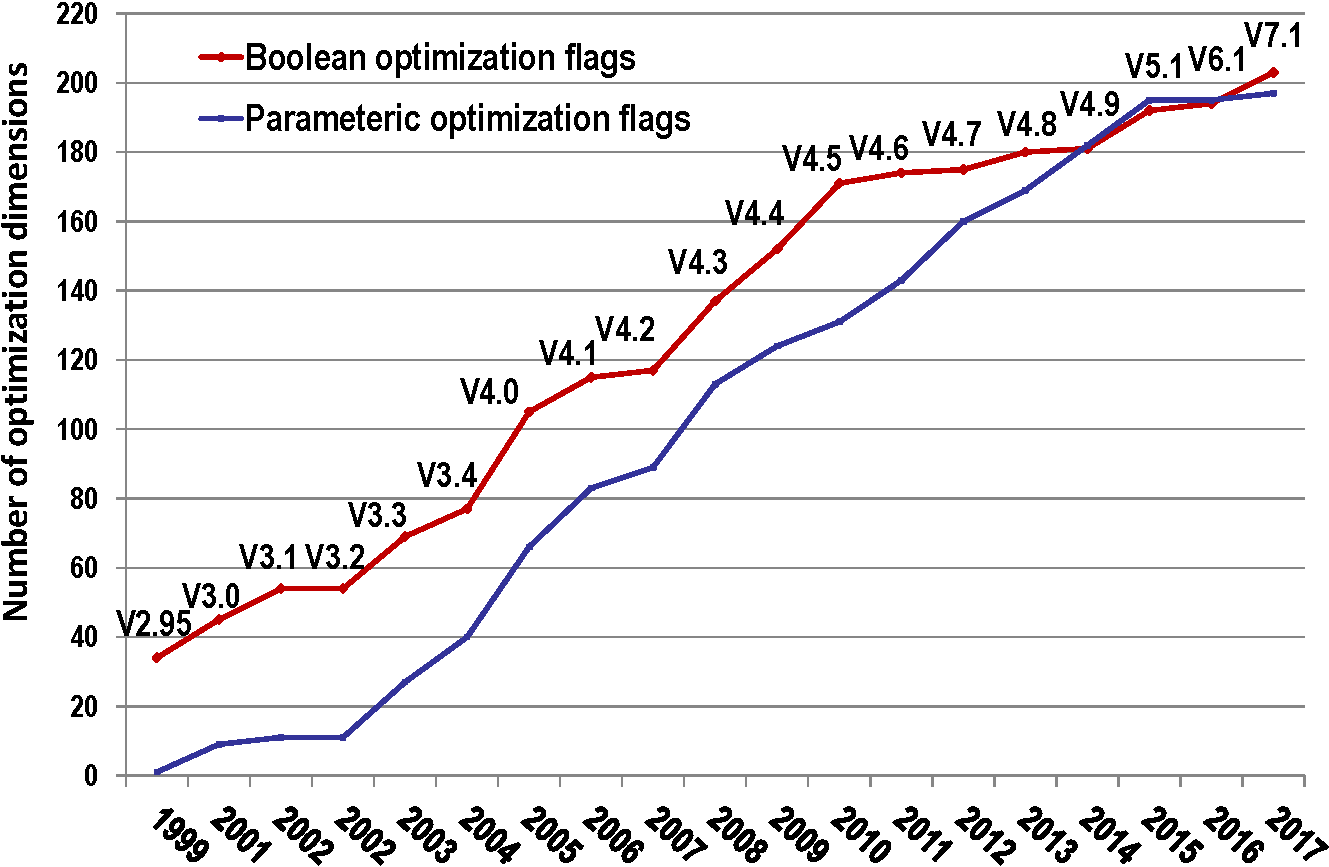
\includegraphics[width=3.4in]
      {ck-assets/aaf72841d69bde12-cropped.pdf} %CK_URL={aaf72841d69bde12-cropped.pdf}
     \caption{
       Continuously rising number of boolean and parametric optimization flags 
       in GCC over years (obtained by automatically parsing GCC source code 
       and manual pages, therefore small variation is possible).
     }
     \label{fig:rising-compiler-flags}
   \end{figure}

Our idea is to keep compiler as a simple collection of code analysis and transformation routines 
and separate it from optimization heuristics.
%
In such case we can use CK autotuning workflow to collaboratively optimize multiple 
shared benchmarks and realistic workloads across diverse hardware, exchange optimization results,
and continuously learn and update compiler optimization heuristics for a given hardware 
as a compiler plugin.
%
We will demonstrate this approach by randomly optimizing compiler flags 
for \textit{susan corners} program with aging \textit{GCC 4.9.2}, the latest \textit{GCC 7.1.0}
and compare them with~\textit{Clang 3.8.1}.
%
We already monitor and optimize execution time and code size of this popular image processing 
application across different compilers and platforms for many years~\cite{29db2248aba45e59:a31e374796869125}.
%
That is why we are interested to see if we can still improve it with the CK autotuner 
on the latest \textit{Raspberry Pi 3 (Model B)} devices (RPi3) extensively used for educational purposes.

First of all, we added \textit{susan} program with \textit{corners} algorithm 
to the \textit{ctuning-programs} repository with the JSON meta information 
describing compilation and execution 
as shown in Figure~\ref{fig:susan-corners-ck-json-meta}.

   % === susan CK meta ==================================================================
   %CK={"action":"prepare_for_latex", "cid":"slide:678dbc30be21a7ab", "file":"354165ad6dde5667-cropped.pdf", "path":"ck-assets", "ck_image":"yes", "ck_image_width":400}
   \begin{figure}[]
     \centering
      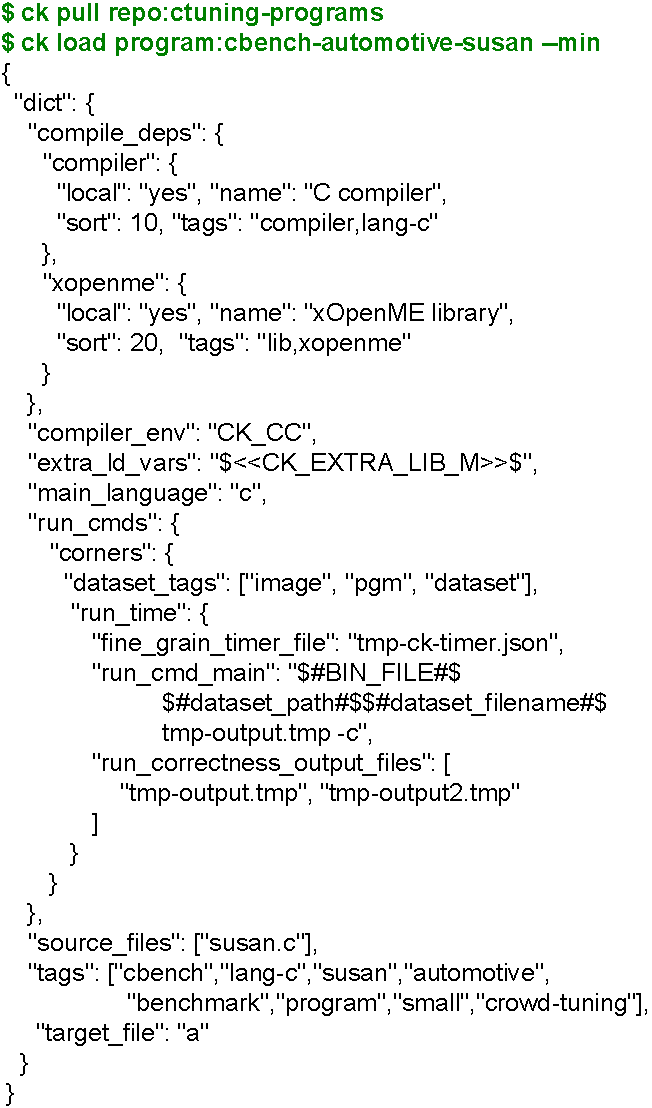
\includegraphics[width=2.8in]
      {ck-assets/354165ad6dde5667-cropped.pdf} %CK_URL={354165ad6dde5667-cropped.pdf}
     \caption{
       CK JSON meta information for susan corners (image processing program) to describe software dependencies as well as how to compile and run it.
     }
     \label{fig:susan-corners-ck-json-meta}
   \end{figure}

We can then test its compilation and execution by invoking the program pipeline as following:
\begin{flushleft}
\texttt{\$ ck pipeline program:cbench-automotive-susan}\newline
\end{flushleft}

CK program pipeline will first attempt to detect platform features
(OS, CPU, GPU) and embed them to the input dictionary using key \textit{features}.
%
Note that in case of cross-compilation for a target platform different from the host one
(Android, remote platform via SSH, etc), 
it is possible to specify such platform using CK \textit{os} entries and \textit{--target\_os=} flag.

For example, it is possible to compile and run a given CK program for Android via adb as following:
\begin{flushleft}
\texttt{\$ ck ls os}\newline
\texttt{\$ ck pipeline program:cbench-automotive-susan --target\_os=android21-arm64}\newline
\end{flushleft}

Next, CK will try to resolve software dependencies and prepare environment for compilation
by detecting already installed compilers using CK \textit{soft:compiler.*} entries 
or installing new ones if none was found using CK \textit{package:compiler.*}.
%
Each installed compiler for each target 
will have an associated CK entry with prepared environment 
to let computer systems researchers work with different 
versions of different tools:
\begin{flushleft}
\texttt{\$ ck show env}\newline
\texttt{\$ ck show env --target\_os=android21-arm64}\newline
\texttt{\$ ck show env --tags=compiler}\newline
\end{flushleft}

Automatically detected version of a selected compiler is used by CK
to find and preload all available optimization flags 
from related \textit{compiler:*} entries to the \textit{choices} key
of a pipeline input.
%
An example of such flags and tags in the CK JSON format 
for GCC 4.9 is shown in Figure~\ref{fig:ck-gcc-meta}.
%
The community can continue extending such descriptions for different compilers
including \textit{GCC, LLVM, Julia, Open64, PathScale, Java, MVCC, ICC and PGI}
using either public \href{https://github.com/ctuning/ck-autotuning}{ck-autotuning} repository
or their own ones.

   % === GCC 4.9 compiler flags meta ==================================================================
   %CK={"action":"prepare_for_latex", "cid":"slide:678dbc30be21a7ab", "file":"84964b0640173783-cropped.pdf", "path":"ck-assets", "ck_image":"yes", "ck_image_width":400}
   \begin{figure}[]
     \centering
      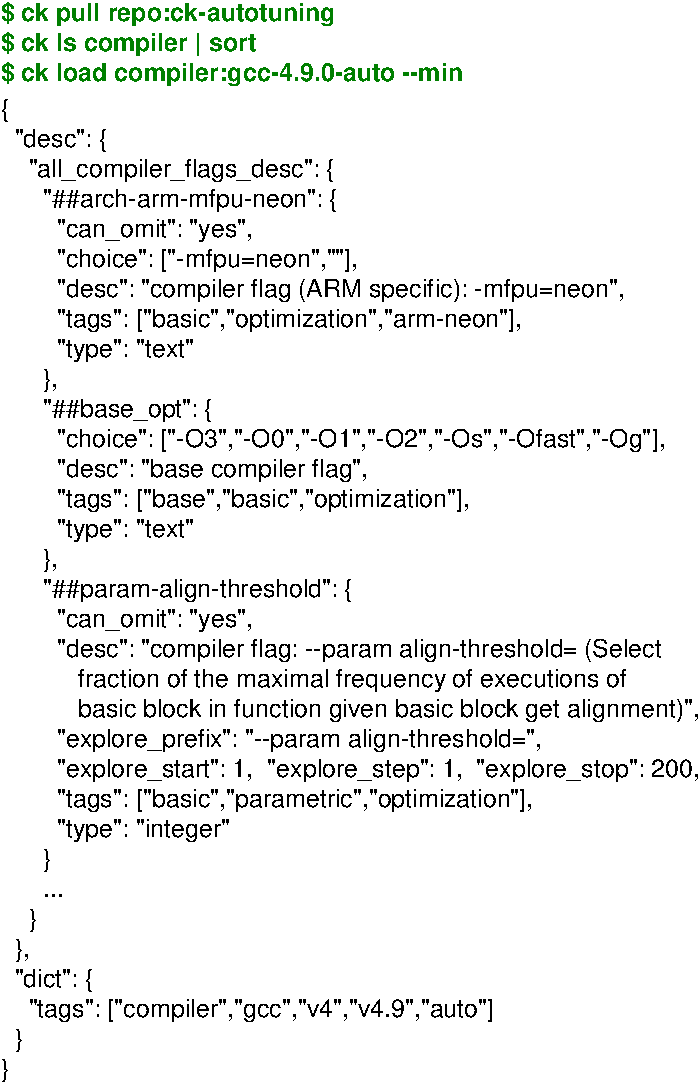
\includegraphics[width=3.0in]
      {ck-assets/84964b0640173783-cropped.pdf} %CK_URL={84964b0640173783-cropped.pdf}
     \caption{
       CK JSON description of compiler flags for GCC 4.9 to enable universal autotuning.
     }
     \label{fig:ck-gcc-meta}
   \end{figure}

Finally, CK program pipeline compiles a given program, runs it on a target platform
and fills in sub-dictionary \textit{characteristics} 
with compilation time, object and binary sizes, MD5 sum of the binary, execution time,
used energy (if supported by a used platform), and all other obtained measurements
in the common pipeline dictionary.

We are now ready to implement universal compiler flag autotuning coupled with
this program pipeline.
%
For a proof-of-concept, we implemented GCC compiler flags exploration strategy
which automatically generate N random combinations of compiler flags, 
compile a given program with each combination, runs it and record all results 
(inputs and outputs of a pipeline) in a reproducible form in a \textit{local} 
CK repository using \textit{experiment} module from 
the \href{https://github.com/ctuning/ck-analytics}{ck-analytics} 
repository:

\begin{flushleft}
\texttt{\$ ck pull repo:ck-crowdtuning}\newline
\texttt{\$ ck info module:experiment.tune.compiler.flags.gcc}\newline
\end{flushleft}

The JSON meta information of this module describes which keys to select
in the program pipeline, how to tune them, and which characteristics to monitor
and record as shown in Figure~\ref{fig:ck-gcc-tuning-meta}.
%
Note that a string starting with \emph{\#\#} is used to reference any key
in a complex, nested JSON or Python dictionary (\textit{CK flat key} \cite{fursin:hal-01054763}).
%
Such \emph{flat key} always starts with \emph{\#} 
followed by \emph{\#key} if it is a dictionary key or
\emph{@position\_in\_a\_list} if it is a value in a list. 
%
CK also supports wild cards in such flat keys 
such as \emph{"\#\#compiler\_flags\#\*"} and \emph{"\#\#characteristics\#\*}
to be able to select multiple sub-keys, dictionaries 
and lists in a given dictionary.


   % === GCC tuning scenario meta ==================================================================
   %CK={"action":"prepare_for_latex", "cid":"slide:678dbc30be21a7ab", "file":"4c2fb19c5b0fd89a-cropped.pdf", "path":"ck-assets", "ck_image":"yes", "ck_image_width":400}
   \begin{figure}[]
     \centering
      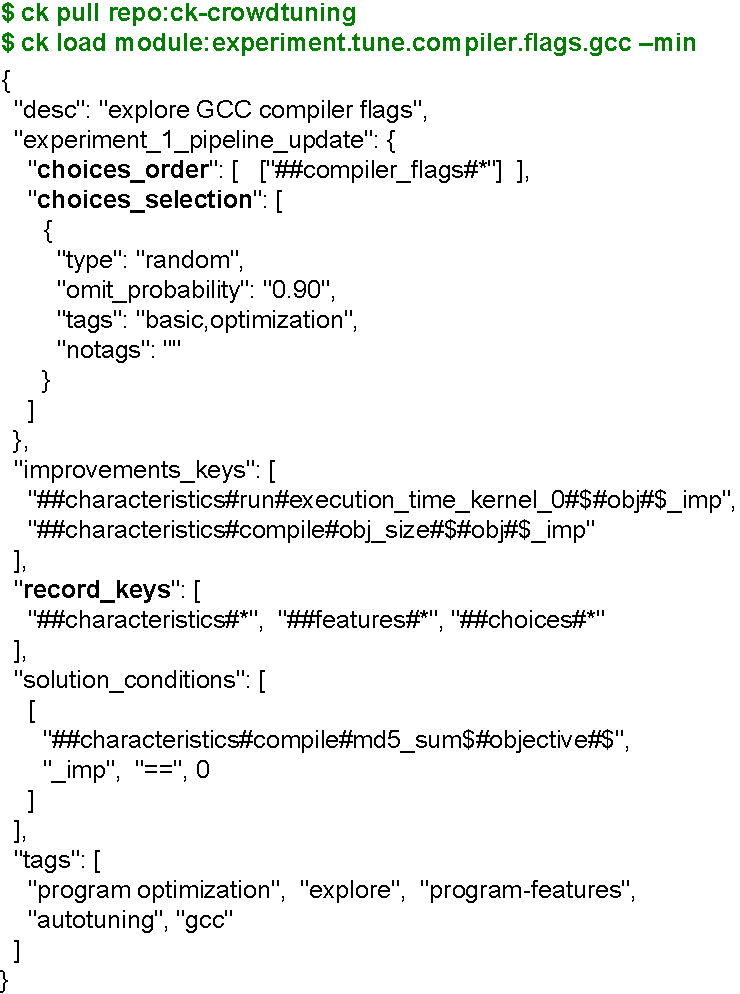
\includegraphics[width=3.0in]
      {ck-assets/4c2fb19c5b0fd89a-cropped.pdf} %CK_URL={4c2fb19c5b0fd89a-cropped.pdf}
     \caption{
       CK JSON description of random autotuning of compiler flags applied to program pipeline.
     }
     \label{fig:ck-gcc-tuning-meta}
   \end{figure}

We can now invoke this CK experimental scenario from the command line as following:

\begin{flushleft}
\texttt{\$ ck autotune program:cbench-automotive-susan --iterations=300 --repetitions=3 
  --scenario=experiment.tune.compiler.flags.gcc
  --cmd\_key=corners --record\_uoa=tmp-susan-corners-gcc4-300-rnd}
\end{flushleft}

CK will generate 300 random combinations of compiler flags, compile \textit{susan corners} program 
with each combination, run each produced code 3 times to check variation, and record
results in the \textit{experiment:tmp-susan-corners-gcc4-300-rnd}.
%
We can now visualize these autotuning results using the following command line:
\begin{flushleft}
\texttt{\$ ck plot graph:tmp-susan-corners-gcc4-300-rnd}
\end{flushleft}

Figure~\ref{fig:autotuning-susan-gcc4} shows a manually annotated graph 
with the outcome of GCC 4.9.2 random compiler flags autotuning 
applied to susan corners on an RPi3 device in terms of execution 
time with variation and code size.
%
Each blue point on this graph is related to one combination of random compiler flags.
%
The red line highlights the frontier of all autotuning results (not necessarily Pareto optimal) 
which trade off execution time and code size during multi-objective optimization.
%
We also plotted points when default GCC compilation is used without any flags 
or with \textit{-O3} and \textit{-Os} optimization levels.
%
Finally, we decided to compare optimization results with \textit{Clang 3.8.1} also available on RPi3.

  % === GCC 4.9.2 ==================================================================
  %CK={"action":"prepare_for_latex", "cid":"slide:3d77e1e8eb6a4b26", "file":"4373f49dea7663db-cropped.pdf", "path":"ck-assets", "ck_image":"yes", "ck_image_width":900}
  %CK={"action":"prepare_for_latex", "cid":"slide:3d77e1e8eb6a4b26", "file":"4373f49dea7663db-table1.tex", "uid":"365ac12dd46fbb42", "path":"ck-assets"}
  %CK={"action":"prepare_for_latex", "cid":"slide:3d77e1e8eb6a4b26", "file":"4373f49dea7663db-table1.html", "uid":"365ac12dd46fbb42", "path":"ck-assets"}
  \begin{figure*}[!htbp]
    \centering
     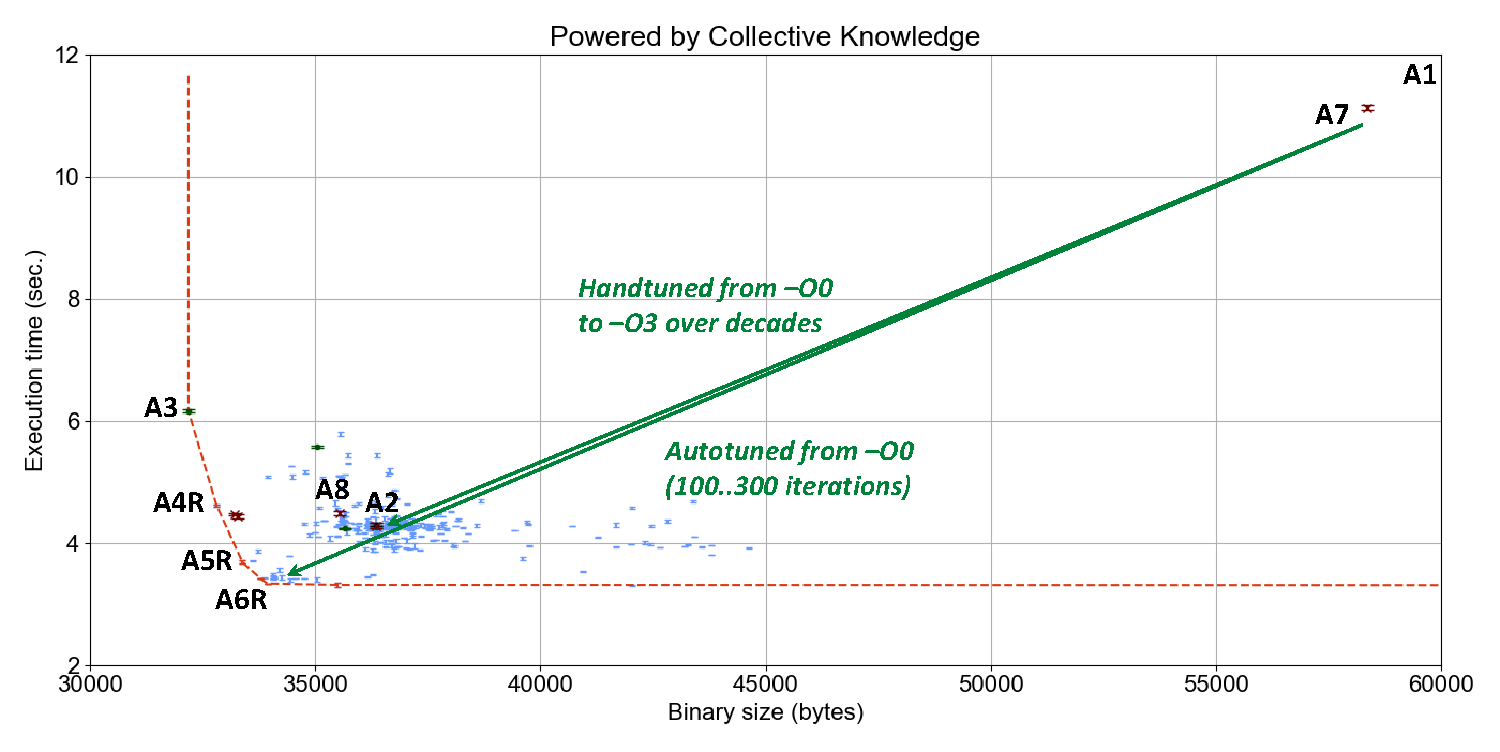
\includegraphics[width=6.9in]
     {ck-assets/4373f49dea7663db-cropped.pdf} %CK_URL={4373f49dea7663db-cropped.pdf}
     \vspace{0.1in}
         \begin{tabular}{|l|l|l|l|p{3.2in}|}
     \hline
      \textbf{ID} & \textbf{Compiler} & \textbf{Time (sec.)} & \textbf{Size (bytes)} & \textbf{Flags} \\ 
     \hline
      \textbf{ \href{http://cknowledge.org/repo/web.php?wcid=experiment:f9e6ec8d198c36c3\&subpoint=7cf654adb86fb606}{A1} } &  GCC 4.9.2  &  11.7 $\pm$ 0.0  &  60560  & {\small  }\\
     \hline
      \textbf{ \href{http://cknowledge.org/repo/web.php?wcid=experiment:0b867dd820354a8b\&subpoint=5734f47e4214a783}{A2} } &  GCC 4.9.2  &  4.3 $\pm$ 0.1  &  36360  & {\small -O3 }\\
     \hline
      \textbf{ \href{http://cknowledge.org/repo/web.php?wcid=experiment:b2b26ab783304fc4\&subpoint=7d87c22a2425da10}{A3} } &  GCC 4.9.2  &  6.2 $\pm$ 0.1  &  32184  & {\small -Os }\\
     \hline
      \textbf{ \href{http://cknowledge.org/repo/web.php?wcid=experiment:98688a71f99ac30b\&subpoint=4bcd9dad6b249a79}{A4R} } &  GCC 4.9.2  &  4.2 $\pm$ 0.0  &  32448  & {\small -O3 -fno-guess-branch-probability -fno-if-conversion -fno-ivopts -fno-schedule-insns -fsingle-precision-constant --param max-unswitch-insns=5 }\\
     \hline
      \textbf{ \href{http://cknowledge.org/repo/web.php?wcid=experiment:984b2d8abc3c4415\&subpoint=78c281b4cab897a6}{A5R} } &  GCC 4.9.2  &  3.7 $\pm$ 0.1  &  33376  & {\small -O3 -fbranch-probabilities -fno-ivopts -fno-sched-dep-count-heuristic }\\
     \hline
      \textbf{ \href{http://cknowledge.org/repo/web.php?wcid=experiment:7af17ca204080b57\&subpoint=5a464ecf81b60098}{A6R} } &  GCC 4.9.2  &  3.4 $\pm$ 0.0  &  33804  & {\small -O3 -fno-inline-small-functions -fno-ivopts -fno-tree-partial-pre }\\
     \hline
      \textbf{ \href{http://cknowledge.org/repo/web.php?wcid=experiment:a32e34c31b900930\&subpoint=64ec888d2e6a0669}{A8} } &  CLANG 3.8.1  &  11.1 $\pm$ 0.1  &  58368  & {\small  }\\
     \hline
      \textbf{ \href{http://cknowledge.org/repo/web.php?wcid=experiment:99141b3313132494\&subpoint=a63f42ac837e38d0}{A9} } &  CLANG 3.8.1  &  4.5 $\pm$ 0.1  &  35552  & {\small -O3 }\\
     \hline
    \end{tabular}     %CK_HTML={ck-assets/4373f49dea7663db-table1.html}
     \vspace{0.1in}
    %CK_INTERACTIVE_GRAPH_PASSIVE={"cid":"2d41f89bcf32d4d4:6b6d77a51c74ec1a", "where":"div#ck_interactive_98fd5cefd4ef2b27", "html":"rpi3-autotuning-susan-gcc4-interactive.html", "style":"rpi3-autotuning-susan-gcc4-interactive.style", "add_div":"yes", "add_box":"yes", "box_width":700, "remove_script_src":"no"}
    \caption{
      Results of GCC 4.9.2 random compiler flag autotuning of susan corners program on Raspberry~Pi~3 (Model~B) 
      device using CK with a highlighted frontier (trading-off execution time and code size) 
      and best found combinations of flags on this frontier.
    }
    \label{fig:autotuning-susan-gcc4}
  \end{figure*}

Besides showing that \textit{GCC -O3} (optimization choice \textbf{A2})
and \textit{Clang -O3} (optimization choice \textbf{A8}) can produce a very similar code, 
these results confirm well that it is indeed possible to automatically obtain execution time 
and binary size of \textit{-O3} and \textit{-Os} levels in comparison with non-optimized code 
within tens to hundreds autotuning iterations (green improvement vectors with ~3.6x execution time speedup 
and ~1.6x binary size improvement).
%
The graph also shows that it is possible to improve best optimization level \textit{-O3} 
much further and obtain ~1.3x execution time speedup (optimization solution \textbf{A6R}
or obtain 11\% binary size improvement without sacrifying original execution time
(optimization solution \textbf{A4R}).
%
Such automatic squeezing of a binary size without sacrificing performance 
can be very useful for the future IoT devices.

Note that it is possible to browse all results in a user-friendly way 
via web browser using the following command:

\begin{flushleft}
\texttt{\$ ck browse experiment:tmp-susan-corners-gcc4-300-rnd}
\end{flushleft}

CK will then start internal CK web server 
available in the \href{https://github.com/ctuning/ck-web}{ck-web}
repository, will run a default web browser, and will 
open a web page with all given experimental results.
%
Each experiment on this page has an associated button 
with a command line to replay it via CK such as:                          

\begin{flushleft}
\texttt{\$ ck replay experiment:7b41a4ac1b3b4f2b --point=00e81f4e4abb371d}
\end{flushleft}

CK will then attempt to reproduce this experiment using the same input
and then report any differences in the output.
%
This simplifies validation of shared experimental results 
(optimizations, models, bugs) by the community
and possibly with a different software and hardware setup
(CK will automatically adapt the workflow to a user platform).

We also provided support to help researchers 
visualize their results as interactive graphs 
using popular D3.js library as demonstrated in this 
\href{http://cknowledge.org/repo/web.php?wcid=graph:6b6d77a51c74ec1a&subgraph=rpi3-autotuning-susan-gcc4-interactive}{link}.

Looking at above optimization results one may notice 
that one of the original optimization solutions on a frontier \textbf{A4} 
has ~40 optimization flags, while \textbf{A4R} only 7 as shown in Table~\ref{fig:autotuning-susan-gcc4-reduce}.
%
The natural reason is that not all randomly selected flags contribute to improvements.
%
That is why we developed a simple and universal complexity reduction algorithm.
%
It iteratively and randomly removes choices from a found solution one by one
if they do not influence monitored characteristics such as execution time and code size
in our example.

  % === GCC 4.9.2 complexity reduction ==================================================================
  %CK={"action":"prepare_for_latex", "cid":"slide:3d77e1e8eb6a4b26", "file":"4373f49dea7663db-table2.tex", "uid":"a4f68aabe479b46b", "path":"ck-assets"}
  %CK={"action":"prepare_for_latex", "cid":"slide:3d77e1e8eb6a4b26", "file":"4373f49dea7663db-table2.html", "uid":"a4f68aabe479b46b", "path":"ck-assets"}
  \begin{table*}[]
    \centering
         \begin{tabular}{|l|p{6.2in}|}
     \hline
      \textbf{ID} & \textbf{Flags} \\ 
     \hline
      \textbf{ A4 } & {\small -O3 -fira-algorithm=priority -fcaller-saves -fno-devirtualize-speculatively -fno-function-cse -fgcse-sm -fno-guess-branch-probability -fno-if-conversion -fno-inline-functions-called-once -fipa-reference -fno-ira-loop-pressure -fira-share-save-slots -fno-isolate-erroneous-paths-dereference -fno-ivopts -floop-nest-optimize -fmath-errno -fmove-loop-invariants -fsched-last-insn-heuristic -fsched2-use-superblocks -fno-schedule-insns -fno-signed-zeros -fsingle-precision-constant -fno-tree-sink -fno-unsafe-loop-optimizations --param asan-instrument-reads=1 --param gcse-unrestricted-cost=5 --param l1-cache-size=11 --param large-function-growth=33 --param loop-invariant-max-bbs-in-loop=636 --param max-completely-peel-loop-nest-depth=7 --param max-delay-slot-live-search=163 --param max-gcse-insertion-ratio=28 --param max-inline-insns-single=282 --param max-inline-recursive-depth-auto=0 --param max-jump-thread-duplication-stmts=6 --param max-last-value-rtl=4062 --param max-pipeline-region-insns=326 --param max-sched-region-blocks=17 --param max-tail-merge-iterations=2 --param max-unswitch-insns=5 --param max-vartrack-expr-depth=6 --param min-spec-prob=1 --param omega-eliminate-redundant-constraints=1 --param omega-max-keys=366 --param omega-max-wild-cards=36 --param sms-dfa-history=0 }\\
     \hline
      \textbf{ A4R } & {\small -O3 -fno-guess-branch-probability -fno-if-conversion -fno-ivopts -fno-schedule-insns -fsingle-precision-constant --param max-unswitch-insns=5 }\\
     \hline
    \end{tabular}     %CK_HTML={ck-assets/4373f49dea7663db-table2.html}
    \caption{
      One of original optimization solutions found after autotuning with random selection of compiler flags (A4) 
      and reduced optimization solution (A4R) which results in the same or better execution time and code size.
    }
    \label{fig:autotuning-susan-gcc4-reduce}
  \end{table*}

Such complexity reduction (pruning) of an existing solution can be invoked as following
(flag \textit{--prune\_md5} tells CK to exclude a given choice without running code
if MD5 of a produced binary didn't change, thus considerably speeding up flag pruning):

\begin{flushleft}
\texttt{\$ck replay experiment:93974bf451f957eb --point=74e9c9f14b424ba7 --prune --prune\_md5 @prune.json}
\end{flushleft}

The \textit{'prune.json'} file describes conditions on program pipeline keys 
when a given choice should be removed as shown in Figure~\ref{fig:ck-pruning-meta}.

   % === GCC complexity reduction ==================================================================
   %CK={"action":"prepare_for_latex", "cid":"slide:678dbc30be21a7ab", "file":"e2a106816a4c5093-cropped.pdf", "path":"ck-assets", "ck_image":"yes", "ck_image_width":400}
   \begin{figure}[]
     \centering
      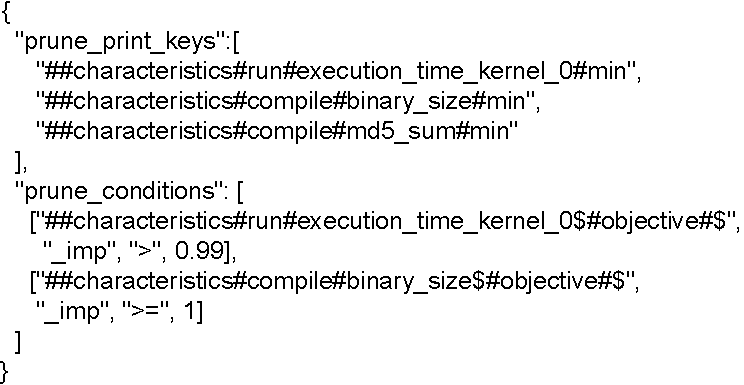
\includegraphics[width=3.0in]
      {ck-assets/e2a106816a4c5093-cropped.pdf} %CK_URL={e2a106816a4c5093-cropped.pdf}
     \caption{
       CK JSON description of conditions on choices in a pipeline input to reduce choices from a found optimization solution.
     }
     \label{fig:ck-pruning-meta}
   \end{figure}

Such universal complexity reduction approach helps software engineers better understand
individual contribution of each flag to improvements or degradations of all monitored
characteristics such as execution time and code size as shown in Figure~\ref{fig:ck-pruning-contribution}.

   % === Pruning contribution  ==================================================================
   %CK={"action":"prepare_for_latex", "cid":"slide:678dbc30be21a7ab", "file":"a472d964631c80a2-cropped.pdf", "path":"ck-assets", "ck_image":"yes", "ck_image_width":400}
   \begin{figure}[]
     \centering
      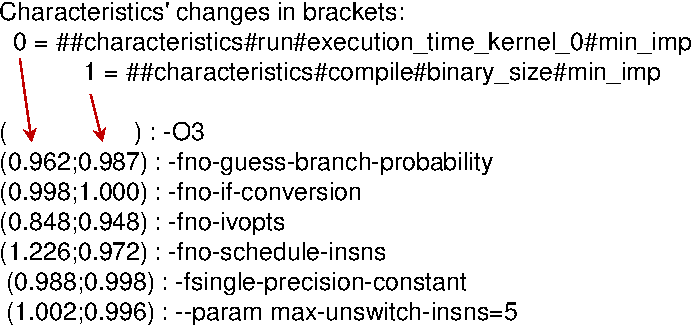
\includegraphics[width=3.0in]
      {ck-assets/a472d964631c80a2-cropped.pdf} %CK_URL={a472d964631c80a2-cropped.pdf}
     \caption{
       Contribution of individual compiler flags to improvements or degradations of monitored characteristics during universal complexity reduction.
     }
     \label{fig:ck-pruning-contribution}
   \end{figure}

Asked by compiler developers, we also provided an extension to our complexity reduction module 
to turn off explicitly all available optimization choices one by one
if they do not influence found optimization result.
%
Table~\ref{fig:autotuning-susan-gcc4-invert} demonstrates this approach and shows all compiler optimizations contributing to the found optimization solution.
%
It can help improve internal optimization heuristics, global optimization levels such as \textit{-O3},
and improve machine learning based optimization predictions.
%
This extension can be invoked by adding flags \textit{--prune\_invert --prune\_invert\_do\_not\_remove\_key}
when reducing complexity of a given solution such as:
\begin{flushleft}
\texttt{\$ ck replay experiment:93974bf451f957eb --point=74e9c9f14b424ba7 --prune --prune\_md5 --prune\_invert --prune\_invert\_do\_not\_remove\_key @prune.json}
\end{flushleft}

  % === GCC 4.9.2 invertion ==================================================================
  %CK={"action":"prepare_for_latex", "cid":"slide:3d77e1e8eb6a4b26", "file":"4373f49dea7663db-table3.tex", "uid":"ec969fa033ed462b", "path":"ck-assets"}
  %CK={"action":"prepare_for_latex", "cid":"slide:3d77e1e8eb6a4b26", "file":"4373f49dea7663db-table3.html", "uid":"ec969fa033ed462b", "path":"ck-assets"}
  \begin{table*}[]
   \centering
        \begin{tabular}{|l|p{6.2in}|}
     \hline
      \textbf{ID} & \textbf{Flags} \\ 
     \hline
      \textbf{ \href{http://cknowledge.org/repo/web.php?wcid=experiment:7af17ca204080b57\&subpoint=5a464ecf81b60098}{A6R} } & {\small -O3 -fno-inline-small-functions -fno-ivopts -fno-tree-partial-pre }\\
     \hline
      \textbf{ \href{http://cknowledge.org/repo/web.php?wcid=experiment:f594f90a1545babf\&subpoint=de11e85953947388}{A6RI} } & {\small \textbf{-O3} -fno-inline-small-functions -fno-ivopts -fno-tree-bit-ccp -fno-tree-partial-pre -fno-tree-pta -fno-associative-math -fno-auto-inc-dec -fno-branch-probabilities -fno-branch-target-load-optimize -fno-branch-target-load-optimize2 -fno-caller-saves -fno-check-data-deps -fno-combine-stack-adjustments -fno-conserve-stack -fno-compare-elim \textbf{-fcprop-registers} \textbf{-fcrossjumping} \textbf{-fcse-follow-jumps} -fno-cse-skip-blocks -fno-cx-limited-range -fno-data-sections \textbf{-fdce} -fno-delayed-branch -fno-devirtualize -fno-devirtualize-speculatively -fno-early-inlining -fno-ipa-sra -fno-expensive-optimizations -fno-fat-lto-objects -fno-fast-math -fno-finite-math-only -fno-float-store \textbf{-fforward-propagate} -fno-function-sections -fno-gcse-after-reload -fno-gcse-las -fno-gcse-lm -fno-graphite-identity -fno-gcse-sm -fno-hoist-adjacent-loads -fno-if-conversion \textbf{-fif-conversion2} -fno-indirect-inlining -fno-inline-functions -fno-inline-functions-called-once -fno-ipa-cp -fno-ipa-cp-clone -fno-ipa-pta \textbf{-fipa-pure-const} -fno-ipa-reference -fno-ira-hoist-pressure -fno-ira-loop-pressure -fno-ira-share-save-slots \textbf{-fira-share-spill-slots} \textbf{-fisolate-erroneous-paths-dereference} -fno-isolate-erroneous-paths-attribute -fno-keep-inline-functions -fno-keep-static-consts -fno-live-range-shrinkage -fno-loop-block -fno-loop-interchange -fno-loop-strip-mine -fno-loop-nest-optimize -fno-loop-parallelize-all -fno-lto -fno-merge-all-constants -fno-merge-constants -fno-modulo-sched -fno-modulo-sched-allow-regmoves \textbf{-fmove-loop-invariants} -fno-branch-count-reg -fno-defer-pop -fno-function-cse \textbf{-fguess-branch-probability} \textbf{-finline} \textbf{-fmath-errno} -fno-peephole \textbf{-fpeephole2} -fno-sched-interblock -fno-sched-spec -fno-signed-zeros -fno-toplevel-reorder -fno-trapping-math -fno-zero-initialized-in-bss \textbf{-fomit-frame-pointer} -fno-optimize-sibling-calls -fno-partial-inlining -fno-peel-loops -fno-predictive-commoning -fno-prefetch-loop-arrays -fno-ree -fno-rename-registers \textbf{-freorder-blocks} -fno-reorder-blocks-and-partition -fno-rerun-cse-after-loop -fno-reschedule-modulo-scheduled-loops -fno-rounding-math -fno-sched2-use-superblocks \textbf{-fsched-pressure} -fno-sched-spec-load -fno-sched-spec-load-dangerous -fno-sched-group-heuristic \textbf{-fsched-critical-path-heuristic} -fno-sched-spec-insn-heuristic -fno-sched-rank-heuristic -fno-sched-dep-count-heuristic \textbf{-fschedule-insns} \textbf{-fschedule-insns2} -fno-section-anchors -fno-selective-scheduling -fno-selective-scheduling2 -fno-sel-sched-pipelining -fno-sel-sched-pipelining-outer-loops -fno-shrink-wrap -fno-signaling-nans -fno-single-precision-constant -fno-split-ivs-in-unroller -fno-split-wide-types -fno-strict-aliasing \textbf{-fstrict-overflow} -fno-tracer -fno-tree-builtin-call-dce -fno-tree-ccp \textbf{-ftree-ch} -fno-tree-coalesce-vars -fno-tree-copy-prop \textbf{-ftree-copyrename} \textbf{-ftree-dce} \textbf{-ftree-dominator-opts} -fno-tree-dse \textbf{-ftree-forwprop} -fno-tree-fre -fno-tree-loop-if-convert -fno-tree-loop-if-convert-stores \textbf{-ftree-loop-im} -fno-tree-phiprop -fno-tree-loop-distribution -fno-tree-loop-distribute-patterns -fno-tree-loop-linear \textbf{-ftree-loop-optimize} -fno-tree-loop-vectorize -fno-tree-pre \textbf{-ftree-reassoc} -fno-tree-sink \textbf{-ftree-slsr} \textbf{-ftree-sra} -fno-tree-switch-conversion -fno-tree-tail-merge \textbf{-ftree-ter} -fno-tree-vectorize \textbf{-ftree-vrp} -fno-unit-at-a-time -fno-unroll-all-loops -fno-unroll-loops -fno-unsafe-loop-optimizations -fno-unsafe-math-optimizations -fno-unswitch-loops -fno-variable-expansion-in-unroller -fno-vect-cost-model -fno-vpt -fno-web -fno-whole-program -fno-wpa \textbf{-fexcess-precision=standard} \textbf{-ffp-contract=off} \textbf{-fira-algorithm=CB} \textbf{-fira-region=all} }\\
     \hline
    \end{tabular}     %CK_HTML={ck-assets/4373f49dea7663db-table3.html}
   \caption{
     Explicitly switching off all compiler flags one by one if they do not influence the optimization result - 
     useful to understand all compiler optimizations which contributed to the found solution. 
   }
   \label{fig:autotuning-susan-gcc4-invert}
  \end{table*}

We have been analyzing already aging \textit{GCC 4.9.2} because 
it is still the default compiler for Jessy Debian distribution on RPi3.
%
However, we would also like to check how our universal autotuner
works with the latest \textit{GCC 7.1.0}.

Since there is no yet a standard Debian GCC 7.1.0 package available for RPi3,
we need to build it from scratch.
%
This is not a straightforward task since we have to pick up correct 
configuration flags which will adapt GCC build to quite outdated RPi3 libraries.
%
However, once we manage to do it, we can automate this process
using CK \textit{package} module. 

We created a public \href{https://github.com/ctuning/ck-dev-compilers}{ck-dev-compilers} repository
to automate building and installation of various compilers including GCC and LLVM via CK.
%
It is therefore possible to install GCC 7.1.0 on RPi3 as following 
(see Appendix or GitHub repository ReadMe file for more details):

\begin{flushleft}
\texttt{\$ ck pull repo:ck-dev-compilers \newline
\$ ck install package:compiler-gcc-any-src-linux-no-deps --env.PARALLEL\_BUILDS=1 --env.GCC\_COMPILE\_CFLAGS=-O0 --env.GCC\_COMPILE\_CXXFLAGS=-O0 --env.EXTRA\_CFG\_GCC=--disable-bootstrap --env.RPI3=YES --force\_version=7.1.0}
\end{flushleft}

This CK package has an \textit{install.sh} script which is customized 
using environment variables or \textit{--env} flags to build GCC for a target platform.
%
The JSON meta data of this CK package provides optional software dependencies 
which CK has to resolve before installation (similar to CK compilation).
%
If installation succeeded, you should be able to see two prepared environments
for GCC 4.9.2 and GCC 7.1.0 which now co-exist in the system.

\begin{flushleft}
\texttt{\$ ck show env --tags=gcc}
\end{flushleft}

Whenever we now invoke CK autotuning, CK software and package manager 
will detect multiple available versions of a required software dependency
and will let you choose which compiler version to use.
%

Let us now autotune the same \textit{susan corners} program 
by generating 300 random combinations of \textit{GCC 7.1.0} compiler flags
and record results in the \textit{experiment:tmp-susan-corners-gcc7-300-rnd}:

\begin{flushleft}
\texttt{\$ ck autotune program:cbench-automotive-susan --iterations=300 --repetitions=3 
  --scenario=experiment.tune.compiler.flags.gcc
  --cmd\_key=corners --record\_uoa=tmp-susan-corners-gcc7-300-rnd}
\end{flushleft}

Figure~\ref{fig:autotuning-susan-gcc7} shows the results of such \textit{GCC 7.1.0}
compiler flag autotuning (\textbf{B} points) and compares them 
against \textit{GCC 4.9.2} (\textbf{A} points).
%
Note that this graph is also available in interactive form~\href{http://cknowledge.org/repo/web.php?wcid=graph:96fd8e4c8394b1bc&subgraph=rpi3-autotuning-susan-gcc7-interactive}{online}.

   % === GCC 7.1.0 ==================================================================
   %CK={"action":"prepare_for_latex", "cid":"slide:425697a3a4bf7c31", "file":"9e4b1594d3b99443-cropped.pdf", "path":"ck-assets", "ck_image":"yes", "ck_image_width":900}
   %CK={"action":"prepare_for_latex", "cid":"slide:425697a3a4bf7c31", "file":"9e4b1594d3b99443-table1.tex", "uid":"b0992b9b3f748e2a", "path":"ck-assets"}
   %CK={"action":"prepare_for_latex", "cid":"slide:425697a3a4bf7c31", "file":"9e4b1594d3b99443-table1.html", "uid":"b0992b9b3f748e2a", "path":"ck-assets"}
   \begin{figure*}[]
     \centering
      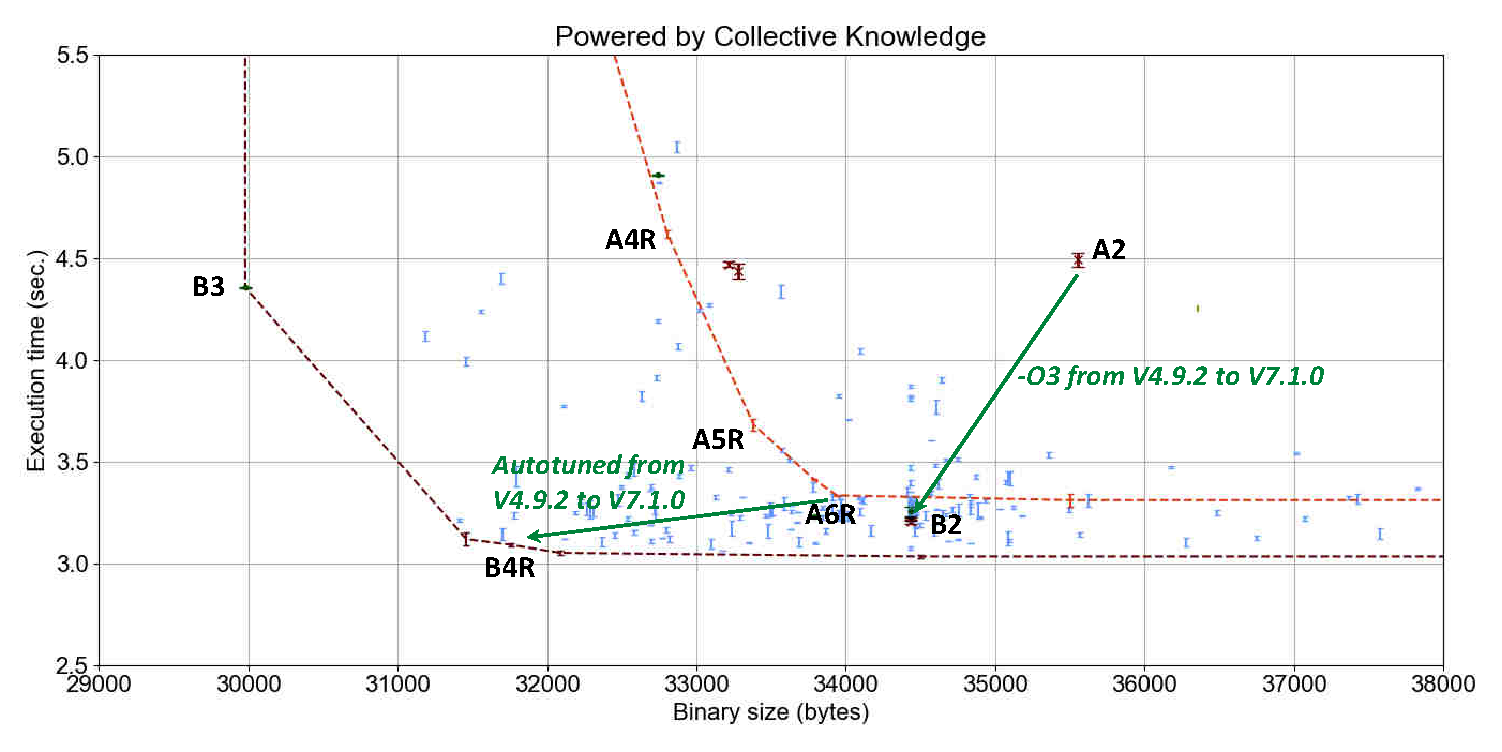
\includegraphics[width=6.9in]
      {ck-assets/9e4b1594d3b99443-cropped.pdf} %CK_URL={9e4b1594d3b99443-cropped.pdf}
      \vspace{0.1in}
          \begin{tabular}{|l|l|l|l|p{3.2in}|}
     \hline
      \textbf{ID} & \textbf{Compiler} & \textbf{Time (sec.)} & \textbf{Size (bytes)} & \textbf{Flags} \\ 
     \hline
      \textbf{ B1 } &  GCC 7.1.0  &  11.5 $\pm$ 0.0  &  58008  & {\small  }\\
     \hline
      \textbf{ B2 } &  GCC 7.1.0  &  3.2 $\pm$ 0.0  &  34432  & {\small -O3 }\\
     \hline
      \textbf{ B3 } &  GCC 7.1.0  &  4.4 $\pm$ 0.0  &  29980  & {\small -Os }\\
     \hline
      \textbf{ B4 } &  GCC 7.1.0  &  3.1 $\pm$ 0.1  &  31460  & {\small -O3 -fno-cx-fortran-rules -fno-devirtualize -fno-expensive-optimizations -fno-if-conversion -fira-share-save-slots -fno-ira-share-spill-slots -fno-ivopts -fno-loop-strip-mine -finline -fno-math-errno -frounding-math -fno-sched-rank-heuristic -fno-sel-sched-pipelining-outer-loops -fno-semantic-interposition -fsplit-wide-types -fno-tree-ccp -ftree-dse }\\
     \hline
      \textbf{ B4R } &  GCC 7.1.0  &  3.1 $\pm$ 0.1  &  31420  & {\small -O3 -fno-expensive-optimizations -fno-ivopts -fno-math-errno }\\
     \hline
    \end{tabular}     %CK_HTML={ck-assets/9e4b1594d3b99443-table1.html}
      \vspace{0.1in}
     \caption{
      Results of GCC 7.1.0 random compiler flag autotuning of susan corners program on Raspberry~Pi~3 (Model~B) 
      device using CK with a highlighted frontier (trading-off execution time and code size), 
      best combinations of flags on this frontier, and comparison with the results from GCC 4.9.2.
     }
     \label{fig:autotuning-susan-gcc7}
   \end{figure*}

It is interesting to see considerable improvement in execution time of susan corners 
when moving from GCC 4.9 to GCC 7.1 with the best optimization level \textit{-O3}.
%
This graph also shows that new optimization added during the past 3 years opened up
many new opportunities thus considerably expanding autotuning frontier (light red
dashed line versus dark red dashed line).
%
Autotuning only managed to achieve a modest improvement of a few percent over \textit{-O3}.

On the other hand, GCC \textit{-O3} and \textit{-Os} are still far from achieving
best trade-offs for execution time and code size.
%
For example, it is still possible to improve a program binary size 
by ~10\% (reduced solution \textbf{B4R}) without degrading best achieved 
execution time with the \textit{-O3} level (\textbf{-O3}), or improve 
execution time of \textbf{-Os} level by ~28\% while slightly degrading code size by ~5\%.

Note that for readers' convenience we added scripts to reproduce and validate 
all results from this section to the following CK entries:

\begin{flushleft}
\texttt{\$ ck pull repo:ck-rpi-optimization-results \newline
\$ ck find script:rpi3-susan*}
\end{flushleft}

These results confirm that it is difficult to manually prepare compiler optimization
heuristic which can deliver good trade offs between execution time and code size 
in such a large design and optimization spaces.
%
They also suggest that either susan corners or similar code 
was eventually added to the compiler regression testing suite,
or some engineer check it manually and fixed compiler heuristic.
%
However, there is also no guarantee that future GCC versions will still
perform well on the susan corners program.
%
Neither these results guarantee that GCC 7.1.0
will perform well on other realistic workloads or devices.
